\documentclass[11pt,a4paper]{article}
\usepackage[T1]{fontenc}\usepackage[utf8]{inputenc}
\usepackage{lmodern,microtype,amsmath,amssymb,amsthm,mathtools}
\usepackage{booktabs,longtable,array,enumitem,xcolor,geometry,fancyhdr,hyperref,graphicx}
\geometry{margin=22mm}
\hypersetup{colorlinks=true,linkcolor=blue!55!black,urlcolor=blue,citecolor=blue!55!black,
 pdftitle={FIN ST1452--ST1541: Structured Uncertainty, Mixture E-Process, Calibration and Refinement Robustness},
 pdfauthor={Krzysztof Żuchowski}}
\pagestyle{fancy}\fancyhf{}\fancyhead[L]{FIN ST1452--ST1541}\fancyhead[R]{Release 11.00}\fancyfoot[C]{\thepage}\setlength{\headheight}{14pt}
\newtheorem{theorem}{Theorem}\newcommand{\status}[1]{\textsf{[#1]}}

\begin{document}
\begin{titlepage}\centering\vspace*{14mm}
{\Huge\bfseries FIN ST1452--ST1541\par}\vspace{4mm}
{\LARGE Structured Uncertainty, Mixture E-Process,\par}\vspace{2mm}
{\LARGE Calibration and Refinement Robustness\par}\vspace{12mm}
{\Large Krzysztof \.Zuchowski\par}
{\normalsize Independent Researcher --- Fractal Information Theory Project\par}
{\normalsize ORCID: 0009-0002-0909-3613\par}\vspace{9mm}
{\large Six research rounds --- 90 programmes\par}
{\large Release 11.00 --- 31 August 2026\par}
\vfill
\begin{minipage}{.87\textwidth}\small
This report extends the interval-certified conditional $OA$ discriminator from
a point decimal spectrum to a structured circulant rounding box, a common
calibration polytope and an exact $12\to24$ coarse refinement.  It also adds a
valid one-sided finite-mixture e-process.  None of these constructions supplies
physical apparatus or selects the state ontology.
\end{minipage}\vfill
{\small English mathematical and computational research report.}
\end{titlepage}

\begin{abstract}
ST1452--ST1541 build a four-level robustness ladder for the conditional FIN
Operational/State discrimination protocol.  First, the point decimal spectrum
of Release 10.99 is replaced by a row-sum-preserving real symmetric circulant
matrix uncertainty model with entry radius $5\times10^{-15}$.  Weyl/row-sum
bounds give eigenvalue radius $6\times10^{-14}$ while preserving Fourier
eigenvectors.  Outward interval replay proves that every admissible spectrum
has one return-gap maximum in the common bracket
$[0.5945307,0.5945309]$.  The global-exclusion margin remains
$3.0895722903\times10^{-6}$, and the four-time composite lower bound remains
\[
\mathrm{RSS}\ge0.04669201121378897.
\]
This is not a theorem for noncirculant perturbations or symbolic kernel
parameters.

A numerical minimax allocation is then studied using the smaller of the two
directional Bernoulli KL divergences.  A finite linear programme assigns
approximately $31.55\%$ of samples to $t=0.3$ and $68.45\%$ to $t=2.0$, with
zero middle-time weights.  Its grid objective is $1.67$ times the equal-
allocation value and survives a finer held-out grid.  Adaptive interval lower
bounds and a two-point dual upper bound certify the continuous minimax value in
$[0.05,0.05370588868619479]$.  The exact optimizing weights remain open; the
four-time design remains the default for the independent RSS theorem.

To repair the invalidity of nuisance likelihood refitting under optional
stopping, a finite 18-component quantum nuisance mixture is frozen.  Each
component likelihood ratio is a martingale under the classical null; their
fixed convex mixture is therefore an e-process.  Crossing 100 rejects the
classical null with anytime Type-I error at most one percent.  The construction
is one-sided and grid-scoped: it does not uniformly accept the classical model
against the continuum.

A common calibration polytope with uniform preparation contamination at most
$5\%$, false-positive/false-negative rates at most $2\%$, and click efficiency
at least $80\%$ preserves at least $91.2\%$ of the ideal gap and yields
\[
\mathrm{RSS}\ge0.03883580017500168.
\]
Independent calibration maps require tighter bounds: the current proof rejects
the $5\%+2\%$ independent budget but accepts a $3\%+2\%$ example.

Finally, the exact Kronecker-sum refinement
\[
A_{24}(q)=A_{12}\otimes I_2+I_{12}\otimes
\begin{pmatrix}q&-q\\-q&q\end{pmatrix}
\]
transports every coarse return, interval certificate and likelihood exactly,
independently of $q$.  A fiber-resolving instrument adds the fine observables
$(1+e^{-2qt})/2$ and $\cos^2(qt)$, but $q$ remains unsourced.  Protocol 11.00
hashes the resulting hierarchy.  Laboratory evidence remains absent.
\end{abstract}

\tableofcontents\newpage

\section{Robustness ladder}

The certification hierarchy is:
\begin{enumerate}
\item exact frozen decimal spectrum;
\item structured row-sum-preserving circulant rounding box;
\item common preparation/detector/loss calibration polytope;
\item exact coarse $12\to24$ refinement.
\end{enumerate}
Each level introduces explicit premises.  Passing a higher level does not
license arbitrary matrix uncertainty, independent instruments or a physical
refinement law.

\section{Round I: ST1452--ST1466 --- structured matrix uncertainty}

Let each independent first-row coefficient of the real symmetric circulant
matrix vary within radius
\[
\delta_A=5\times10^{-15},
\]
subject to exact row-sum zero.  The perturbation remains circulant, so the
Fourier eigenvectors and paired multiplicities are fixed.  The eigenvalue
uncertainty obeys the conservative row-sum/Weyl bound
\[
|\delta\lambda_k|\le12\delta_A=6\times10^{-14}.
\]

The interval proof of Release 10.99 is repeated with these eigenvalue boxes.
Outside $[0.59,0.60]$, the largest Taylor-cover upper bound is
$0.41123791023528017$, while the uncertain candidate lower bound is
$0.41124099980757045$.  The margin is
\[
3.089572290282394\times10^{-6}>0.
\]

On $[0.59,0.60]$,
\[
F''\in[-1.686445990051945,-1.3685959622934722],
\]
so every admissible return-gap curve is strictly concave.  Uniform derivative
signs at $0.5945307$ and $0.5945309$ prove that each curve has one stationary
root in that common bracket.  Consequently every admissible spectrum has its
global maximum inside $[0.59,0.60]$, and its root lies in
$[0.5945307,0.5945309]$.  A common value enclosure has width about
$2.43\times10^{-13}$.

The complete 1000-cell nuisance cover also survives:
\[
\mathrm{RSS}\ge0.04669201121378897,qquad
\max_i|r_i|\ge0.10804167160613187.
\]

\begin{theorem}[structured uncertainty persistence]
The unique time-optimum location and positive four-time composite separation
remain valid throughout the declared symmetric circulant rounding box.
\end{theorem}

The theorem does not cover noncirculant errors, eigenvector rotation or a box
in $(\omega,\phi,\beta,\eta)$.

\section{Round II: ST1467--ST1481 --- time allocation}

For times $T=(0.3,0.6,1.2,2.0)$ and nuisance parameter $\theta=(\alpha,\gamma)$,
define the per-time symmetric design score
\[
d_i(\theta)=\min\{D(C_i\|Q_{i,\theta}),D(Q_{i,\theta}\|C_i)\}.
\]
The finite design problem is
\[
\max_{w_i\ge0,\ \sum_iw_i=1}
\min_{\theta\in\Theta_{\rm grid}}\sum_iw_id_i(\theta).
\]

On a $41\times201$ training grid, linear programming returns
\[
w=(0.3155394972,0,0,0.6844605028),
\]
with objective $0.0537067608$.  Equal allocation gives $0.0322200827$, so the
grid improvement factor is about $1.667$.  A finer independent
$81\times401$ grid has minimum $0.0537030928$ near
$(\alpha,\gamma)=(1.1,16.25)$.

For 100 integer shots, the rounded candidate is $(32,0,0,68)$.  A separate
outward interval cover proves a positive weighted squared-residual lower bound
$0.0046819465$ for these two endpoint times.  Thus exact matching is excluded
on the declared nuisance box.

An adaptive outward cover then subdivides only cells whose analytic rectangular
KL lower bound is below $0.05$.  After 380 splits, 1380 accepted boxes cover the
entire continuous nuisance rectangle and prove that the candidate allocation
has value at least $0.05$.  Conversely, a fixed dual mixture supported at
$(1.1,16)$ and $(1.1,16.25)$ bounds the value of \emph{every} allocation by
$0.05370588868619479$.  Therefore the continuous minimax value for the declared
metric satisfies
\[
0.05\le V_*\le0.05370588868619479.
\]

The exact maximizing weights remain open.  The grid candidate is a certified
near-minimax design, not an exact continuous optimizer.  Its worst case lies on
the clock boundary and the solution lies on a two-time face, making it
sensitive to model-library expansion.  The four-time design remains the
certified conservative default for the independent RSS theorem.

\section{Round III: ST1482--ST1496 --- finite-mixture e-process}

The alternative grid contains
\[
\alpha\in\{0.9,1.0,1.1\},qquad
\gamma\in\{0,5,10,20,50,100\},
\]
for 18 components with uniform weights $\pi_j=1/18$.  For component $j$ let
\[
L_{j,n}=\prod_{i=1}^n\frac{q_j(X_i|t_i)}{p_C(X_i|t_i)}.
\]
Under the classical null every $L_{j,n}$ is a nonnegative mean-one martingale,
and hence
\[
E_n=\sum_{j=1}^{18}\pi_jL_{j,n}
\]
is one.

\begin{theorem}[one-sided mixture test]
Under the frozen classical null,
\[
\Pr_C\left(\sup_nE_n\ge100\right)\le0.01.
\]
The conclusion holds for optional stopping under the predeclared schedule.
\end{theorem}

If component $j$ is true, the mixture obeys $E_n\ge\pi_jL_{j,n}$ and initially
pays at most $\log18$ in log-evidence.  A seeded grid-alternative fixture
crossed the boundary after 32 events; a 500-event classical fixture did not.
These are software tests.

The e-process only supports rejection of $C$ in favour of the frozen mixture.
It does not provide uniformly valid acceptance of $C$ against every component,
and off-grid power is unproved.  A continuous prior mixture is a separate
construction.

\section{Round IV: ST1497--ST1511 --- calibration polytopes}

The common binary calibration map is
\[
T_{\epsilon,a,b}(p)=a+(1-a-b)\left[(1-\epsilon)p+\frac\epsilon{12}\right],
\]
with
\[
0\le\epsilon\le0.05,qquad0\le a,b\le0.02.
\]
When the same map applies to both hypotheses, every return gap is scaled by
\[
g=(1-a-b)(1-\epsilon)\ge0.96\cdot0.95=0.912.
\]
Therefore the base gap remains at least $0.3750310$, and the four-time
certificate becomes
\[
\mathrm{RSS}\ge g^2(0.04669201121378897)
=0.03883580017500168.
\]
At least one residual remains above $0.0985340045$.

If calibration maps may differ by hypothesis, the proof uses the per-model
bound
\[
e_{\rm model}\le\frac{11}{12}\epsilon_{\rm prep}
+\delta_{\rm detector}.
\]
To preserve the certified one-time residual, this must be below
$0.1080416716/2=0.0540208358$.  The independent budget
$\epsilon=0.05$, $\delta=0.02$ gives $0.0658333$ and is not certified.  The
example $0.03+0.02$ gives $0.0475$ and passes.  Failure of the sufficient bound
does not prove actual nonidentifiability.

Known uniform click efficiency $\eta\in[0.8,1]$ preserves click-conditioned
vertex distributions but requires attempts and no-clicks.  The mean attempt
inflation at $eta=0.8$ is $1.25$; this is not a tail guarantee.
Vertex-dependent efficiencies require a stochastic/substochastic detector
matrix polytope and remain open.

\section{Round V: ST1512--ST1526 --- exact refinement transport}

Let
\[
B_q=\begin{pmatrix}q&-q\\-q&q\end{pmatrix},qquad
A_{24}=A_{12}\otimes I_2+I_{12}\otimes B_q.
\]
The commuting Kronecker sum gives
\[
e^{-tA_{24}}=e^{-tA_{12}}\otimes e^{-tB_q},qquad
e^{-itA_{24}}=e^{-itA_{12}}\otimes e^{-itB_q}.
\]

If the instrument sums over the two fiber outcomes at a base node, both
classical and quantum node-return probabilities equal their $12$-state values
for every $q\ge0$ and either initial fiber basis state.  Consequently the
time-optimum certificate, four-time RSS certificate and seven-distance-class
likelihood transport exactly.  The coarse protocol is $q$-blind.

A fiber-resolving measurement supplies additional returns for initial fiber
state $0$:
\[
H_q(t)=\frac{1+e^{-2qt}}2,
\qquad
R_q(t)=\cos^2(qt).
\]
This creates a fine dual-dynamics discriminator.  It requires a 24-outcome or
fiber-resolving calibrated detector and does not derive $q$ or its physical
units.

\begin{figure}[ht]
\centering
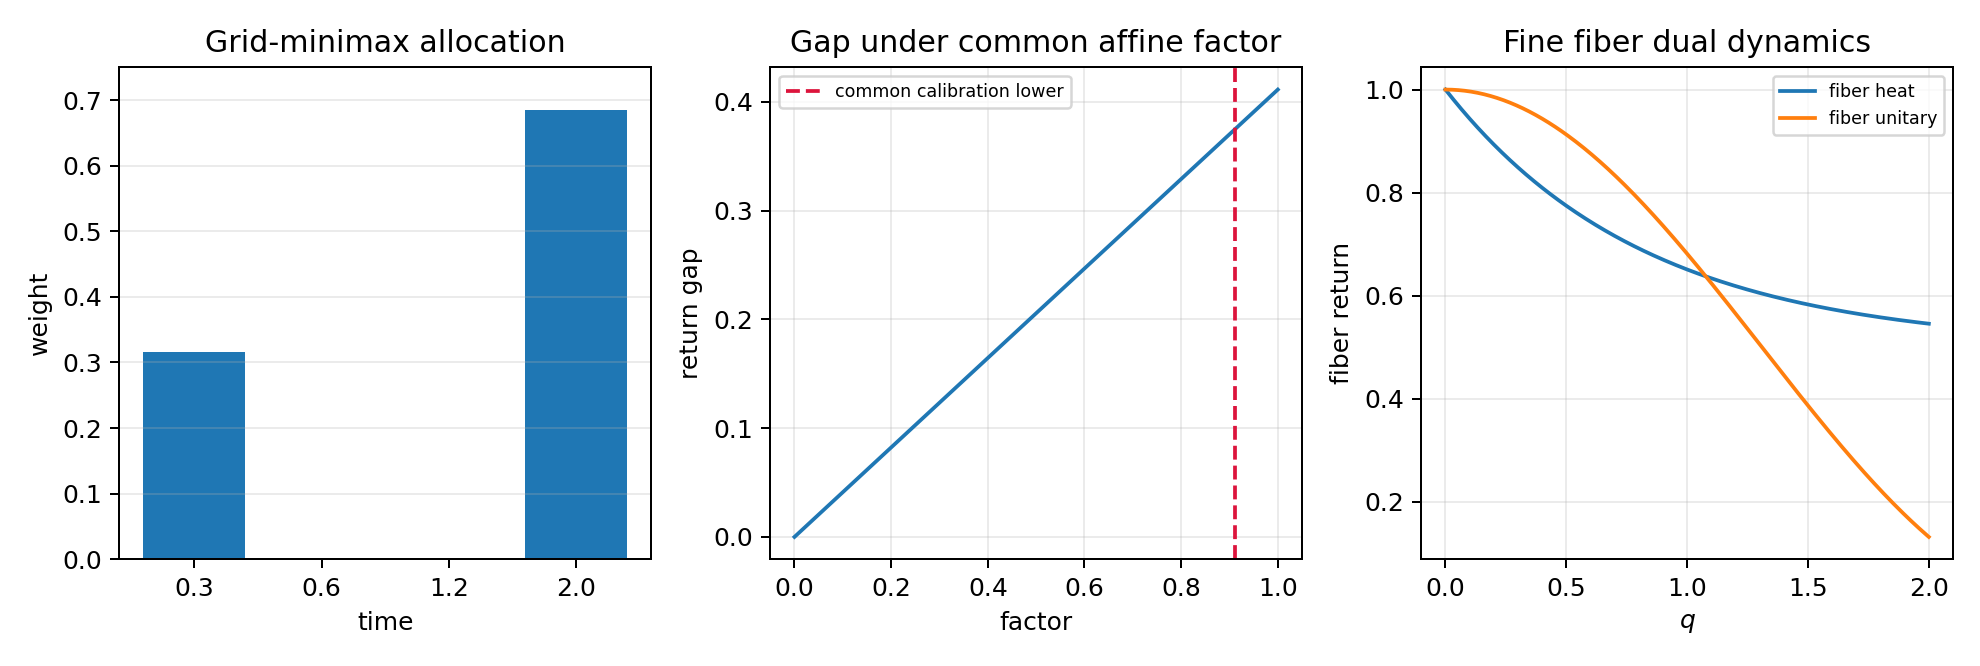
\includegraphics[width=.98\textwidth]{FIN_ST1452_ST1541_Figures/robust_refinement_summary.png}
\caption{Left: numerical grid-minimax time weights.  Centre: return-gap scaling
under a common affine calibration factor.  Right: the optional fine-fiber heat
and unitary returns at $t=0.6$.}
\end{figure}

\section{Round VI: ST1527--ST1541 --- synthesis}

\begin{longtable}{@{}p{.33\textwidth}p{.23\textwidth}p{.34\textwidth}@{}}
\toprule
Layer/result & Status & Boundary \\
\midrule\endhead
structured circulant uncertainty & \status{Interval-proven} & radius $5\times10^{-15}$, Fourier structure fixed \\
KL time allocation & \status{Certified value bracket} & exact optimizing weights open \\
two-time nonidentity & \status{Interval-proven} & weighted squared metric, declared box \\
finite-mixture e-process & \status{Proven one-sided} & 18 frozen components \\
common calibration polytope & \status{Proven} & common affine map \\
independent calibration & \status{Conditional bounds} & $3\%+2\%$ example passes \\
coarse $12\to24$ transport & \status{Exact} & declared Kronecker refinement \\
fine fiber discriminator & \status{Constructed} & $q$ and instrument unsourced \\
laboratory evidence & \status{Absent} & no apparatus/custody/events \\
\bottomrule
\end{longtable}

Protocol \path{FIN_ST1527_ST1541_Protocol_11_00.json} hashes the parent
protocol, mixture grid and calibration polytope, and records the structured
uncertainty, interval bounds, numerical allocation and refinement rule.

These results make one conditional $OA$ discriminator robust across four
explicit layers.  They do not derive a state category, strict clock, physical
detector or the value $q$.

The protocol still tests internal mixing versus coherent dynamics.  It does
not test literal nonexistence of the whole nadsoliton.

\section{Recommended next programmes}

\begin{enumerate}
\item derive interval eigenvector bounds for noncirculant matrix boxes;
\item propagate symbolic $(\omega,\phi,\beta,\eta)$ uncertainty;
\item narrow the continuous KL value bracket and certify optimizing weights;
\item construct a continuous-prior mixture e-process;
\item optimize an independent calibration polytope;
\item certify a vertex-dependent detector matrix box;
\item optimize integer shot allocation;
\item test fine-fiber identifiability of $q$;
\item impose multi-level refinement consistency;
\item derive one platform-specific forward model without claiming realization;
\item freeze external calibration and custody forms;
\item obtain independent review before raw data collection.
\end{enumerate}

Stop if a noncirculant error is treated as circulant, a grid optimum is called
a continuum theorem, mixture rejection is called symmetric decision, a common
calibration proof is applied to independent devices, coarse transport is called
a derivation of $q$, or a synthetic fixture is called evidence.

\section{Final conclusion}

\begin{quote}
The conditional FIN dual-dynamics discriminator is now stable against one
declared structured matrix box, one common calibration polytope and one exact
refinement family.  A finite nuisance mixture also permits valid anytime
rejection of the classical simple null.  The principal remaining mathematical
gap is robustness to noncirculant/eigenvector uncertainty and continuous
nuisance families; the principal physical gap remains an independently
calibrated apparatus and raw event record.
\end{quote}

\appendix
\section{Six-round ledger}
\begin{longtable}{@{}p{.18\textwidth}p{.34\textwidth}p{.38\textwidth}@{}}
\toprule
Range & Object & Verdict \\
\midrule\endhead
ST1452--ST1466 & structured matrix uncertainty & interval certificates survive \\
ST1467--ST1481 & time allocation & continuous value bracket; exact weights open \\
ST1482--ST1496 & mixture e-process & valid one-sided finite-grid rejection \\
ST1497--ST1511 & calibration polytope & common robustness; independent bound split \\
ST1512--ST1526 & refinement transport & exact coarse invariance, fine test \\
ST1527--ST1541 & synthesis & four-level conditional robustness ladder \\
\bottomrule
\end{longtable}

\section{Reproducibility}
The authoritative result sets run from
\path{FIN_ST1452_ST1466_Results.json} through
\path{FIN_ST1527_ST1541_Results.json}.  Each contains fifteen programmes and
packet hashes.  The combined test \path{test_fin_st1452_st1541.py} verifies all
ninety packets, uncertainty margins, allocation status, mixture fail-closed
behaviour, calibration gates, refinement identities, protocol and figure.

\section{Nonclaims}
No arbitrary-matrix or symbolic-kernel interval theorem, continuous minimax
solution, continuous composite e-process, platform calibration, state ontology,
apparatus, raw event, independent custody, legacy bridge, selector, Standard
Model, gravity, $L_{\rm total}$ or Theory of Everything is established.  All
future FIN PDFs remain English.

\begin{thebibliography}{9}
\bibitem{moore} R. E. Moore, R. B. Kearfott and M. J. Cloud, \emph{Introduction to Interval Analysis}, SIAM.
\bibitem{cover} T. M. Cover and J. A. Thomas, \emph{Elements of Information Theory}, Wiley.
\bibitem{ville} J. Ville, \emph{Etude critique de la notion de collectif}, Gauthier-Villars.
\end{thebibliography}
\end{document}
